% \documentclass[12pt,openright,oneside,a4paper,brazil]{abntex2}
% \usepackage[utf8]{inputenc}
% \counterwithout{section}{section}
% \counterwithout{figure}{chapter}
% \counterwithout{table}{chapter}
% \setlength{\parindent}{1.3cm}
% \usepackage{indentfirst}
% \setlength{\parskip}{0.2cm}
% \usepackage[bottom=2cm,top=3cm,left=3cm,right=2cm]{geometry}
% \usepackage{graphicx}
% \graphicspath{{figuras/}}
% \usepackage{placeins}
% \usepackage{cite}
% \usepackage{url}
% \usepackage{breakurl}
% \include{bibliografia}
% 
% \makeatletter
% \setlength{\@fptop}{0pt}
% \makeatother
% 
% \begin{document}
% 
% \textual
% \begin{center}
%  {\large Captação de água e materiais estruturais}\\[0.2cm]
%  \end{center}
 
Dentre as inspirações de tecnologia a serem aplicadas no projeto, as que se destacaram foram a Eolewater, MaxWater, Skywater
e Warkawater. As três primeiras se baseiam no \emph{cooling compression}, porém com custos
diferentes \cite{eole} \cite{whisson}.
A Quarta tem custo extremamente baixo se comparado com as outras três tecnologias, por causa da simplicidade dos
materiais que a constituem. Contudo, produz valores significantemente menores de água, além de não gerar energia
para os processos de controle da qualidade da água (WARKA WATER INC, 2014). Por não gerar energia, também descartamos o Skywater.

\begin{figure}[!ht]
\centering
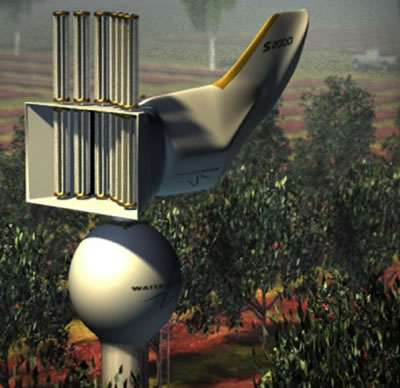
\includegraphics[scale=0.6]{editaveis/figuras/max_water}
\caption[MaxWater]{MaxWater\footnotemark}

\label{max_water_turbina}
\end{figure}
\footnotetext{Disponível em: http://peswiki.com/index.php/Image:Max-water.jpg}

Eole water e max water são turbinas eólicas autossuficientes que retiram a umidade do ar. A geometria dos rotores do MaxWater
não é tão eficiente como os rotores tradicionais, por terem pequeno torque. Além disso, ele ainda não foi testado. Devido a 
insegurança do maxwater, escolhemos como base o sistema da EoleWater, que está retratado na Figura ~\ref{Eole_Water}.

\begin{figure}[!htbp]
\centering
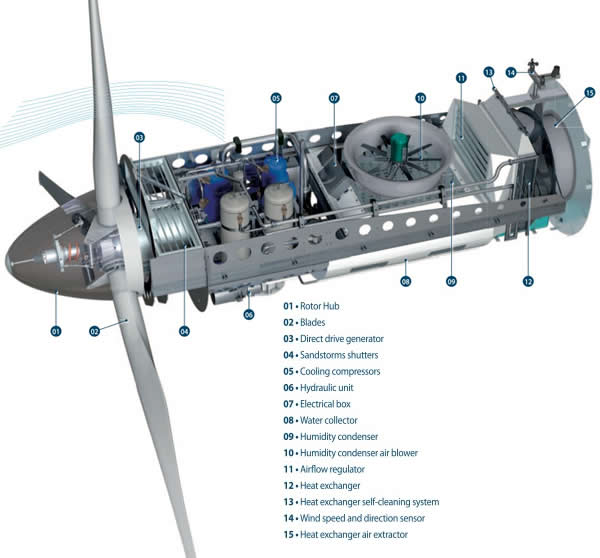
\includegraphics[scale=0.6]{editaveis/figuras/Componentes}
\caption[Componentes de uma turbina Eolewater.]{Componentes de uma turbina Eolewater.\footnotemark}
\FloatBarrier
\label{Eole_Water}
\end{figure}

\footnotetext{Fonte: \cite{renewable} }

Os componentes de uma turbina eólica pouco mudam para essa acima, pois a Eolewater além de gerar energia para seu próprio
funcionamento gera água, enquanto que a turbina eólica gera apenas energia. Na maioria das tecnologias de sucesso que foram alvos de pesquisa,
a obtenção de água é feita pela condensação  a frio (\textit{cooling condensation}), que é feita com o contato de 
ar com uma superfície fria. Para gerar essa superfície fria, um compressor comprime um fluido refrigerante, elevando sua
temperatura. Esse fluido em alta temperatura passa por um trocador de calor e depois é expandido, o que causa uma queda 
ainda maior na temperatura do fluido. O fluido sob baixa temperatura circula por um condensador, por onde passa o ar 
atmosférico coletado. Esse condensador faz com que a temperatura do ar caia até o ponto de orvalho, temperatura na qual a
água presente no ar se condensa em pequenas gotículas devido a saturação da quantidade de água no ar. A água proveniente
da condensação é coletada e passa por tratamentos em UV e carvão ativado para que seja descontaminada e esteja pronta para
consumo.



No momento, o levantamento de materiais será apenas estrutural e se baseará em uma turbina eólica.

\begin{figure}[!htbp]
\centering
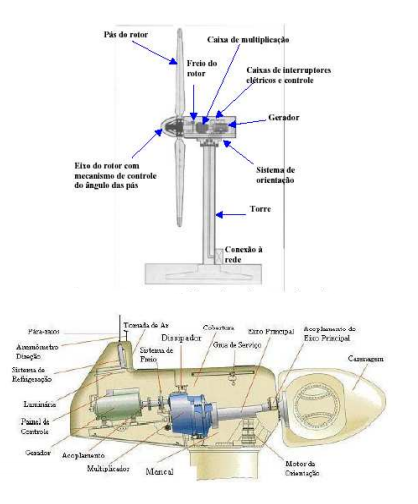
\includegraphics[scale=0.80]{editaveis/figuras/turbina}
\caption[Seção de uma turbina eólica]{Seção de uma turbina eólica típica conectada à rede.\footnotemark}
\FloatBarrier
\label{secao_turbina_eolica}
\end{figure}
\footnotetext{Fonte: USP, 2005 }

Dentro da turbina eólica temos os seguintes subconjuntos: 
\begin{itemize}
\item torre: é um componente que elevará o custo inicial da turbina eólica. Ele tem como funcionalidade sustentar a nacele,
  e todos os seus componentes internos, além de também sustentar o rotor. Essa sustentação permitirá que o sistema trabalhe em
  uma altura adequada ao seu funcionamento.

\item Rotor: transformará a energia proveniente dos ventos (cinética) em energia mecânica, esse mecanismo fixado as pás o qual
  realiza a conversão é chamado de rotor. \cite{rossiEtAl}.

\item Nacele: é a designação a uma estrutura que armazena ou abriga os sistemas matriz da turbina eólica, como os mecanismos do
  gerador (sistemas hidráulicos, embreagens, etc). Usaremos a Nacele para também abrigar os mecanismos de obtenção de água.

\item Caixa multiplicadora: Tem como função transmitir a energia mecânica transformada no rotor para o eixo de rotação do gerador.

\item Gerador: 	A energia transmitida para o eixo de rotação do gerador será transformada em energia elétrica, portanto,
  possui a função de transformar energia mecânica em elétrica.

\item Mecanismos de controle: supervisiona a velocidade média nominal em os ventos chegaram nas pás da turbina, em com qual
  frequência ele irá atuar mediante a um tempo pré-estabelecido.

\item Biruta: 	indicador de direção do vento, também conhecido como \textit{windsock}.

\item Anemômetro: nstrumento capaz de medir a velocidade dos ventos, e também sua intensidade em um intervalo de tempo
  pré-determinado.
  
\item Pás: Estruturas que se movimentarão com o vento e converterão sua potência ao eixo de rotação do rotor, 
  o qual irá fazer a conversão já citada \cite{rossiEtAl}.	 	

\end{itemize}

Um dos componentes que se tem muito estudo é a pá rotativa. Ela pode ser feita com os seguintes materiais: 
madeira, aço, alumínio, fibra de vidro com resina poliéster, fibra de vidro com fibra de carbono, madeira com epóxi,
fibra de carbono. A escolha do material vai depender da escolha do perfil aerodinâmico, que será estudado posteriormente.
\cite{portalEnergia}.

\begin{figure}[!htbp]
\centering
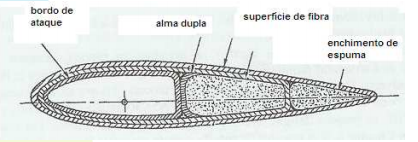
\includegraphics[scale=0.80]{editaveis/figuras/pa}
\caption[Seção transversal de uma pá feita de fibra de vidro]{Seção transversal de uma pá feita de fibra de vidro\footnotemark}
\FloatBarrier
\label{secao_transversal_pa}
\end{figure}
\footnotetext{Fonte: \cite{usp}}

Como pode se visto na imagem acima, as fibras são colocadas nas principais direções onde as tensões atuam quando a turbina
está em operação, região também conhecida como área crítica (longarina da pá). A fibra de carbono e ou Kevlar são atualmente
os compostos mais avançados que podem ser utilizados em áreas críticas (longarina da pá), mas tal material possui preços muito
elevados \cite{barrosVarela}.  

Em relação ao suporte estrutural, ou torre, nas turbinas eólicas elas podem ser do tipo treliçadas, tubular e estaiada,
no entanto, para a Eolewater as estruturas mais comuns são as duas últimas. As torres são constituídas de concreto e aço,
tendo o peso em torno de 40 toneladas e 50 metros de comprimento \cite{usp}.

\begin{figure}[!htb]
\centering
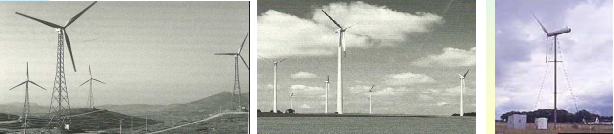
\includegraphics[scale=0.80]{editaveis/figuras/torre}
\caption[Tipos de torre]{Tipos de torre. Da esquerda para a direita: Treliçada, Tubular e Estaiada \footnotemark}
\FloatBarrier
\label{torre}
\end{figure}
\footnotetext{Fonte: \cite{usp}}

O modelo do dispositivo da Eolewater de gerar água por meio da energia eólica possui uma turbina WMS1000, de potência de 30kW.
O tempo de vida proposto para esse mecanismo é de 20 anos, dependendo das condições em que o motor é submetido ele pode gerar
até 1200 litros de água por dia (mais informações na tabela abaixo). Como o dispositivo não necessita de quaisquer outros 
recursos para operar há um impacto mínimo sobre o meio em que é colocado \cite{renewable}.

\begin{figure}[!htbp]
\centering
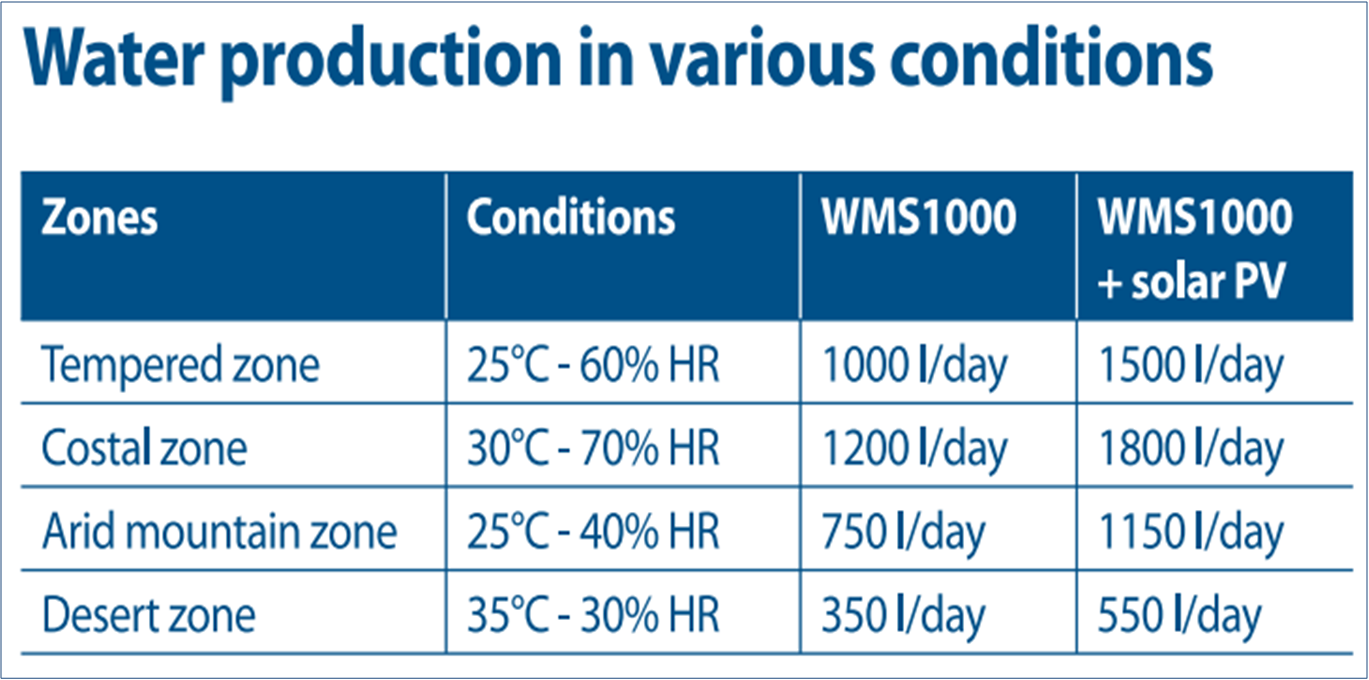
\includegraphics[scale=0.3]{editaveis/figuras/condicoes}
\caption[Tabela de condições de umidade e temperatura para o rendimento de água]{Tabela de condições de umidade e temperatura para o rendimento de água \footnotemark}
\FloatBarrier
\label{condicoes}
\end{figure}
\footnotetext{Fonte: \cite{renewable}}

Essa tecnologia possui um controle de pitch centrífuga para regular a velocidade do motor, tem um sistema de travagem
rotor mecânica e elétrica, o qual evita danos nas lâminas giratórias (pás), ainda, contém um mastro de inclinação que 
integra a ação dos cilindros telescópicos com capacidade de empuxo de 115 toneladas. Deve-se destacar que os componentes 
que entram em contato com a água são feitos de uma liga de aço inoxidável especial que operará sem risco de corrosão 
\cite{eole}.

Uma tecnologia como essa segundo a Eolewater, uma turbina de vento abaixo de 100 kW vai custa por volta de
 US \$ 3.000 a US \$ 5.000 por quilowatt de capacidade \cite{eole}.

Portanto, levando em conta as especificações técnicas do Turbine WMS1000 abaixo a tecnologia é eficiente, mas cara \cite{renewable}.
	
\begin{figure}[!htbp]
\centering
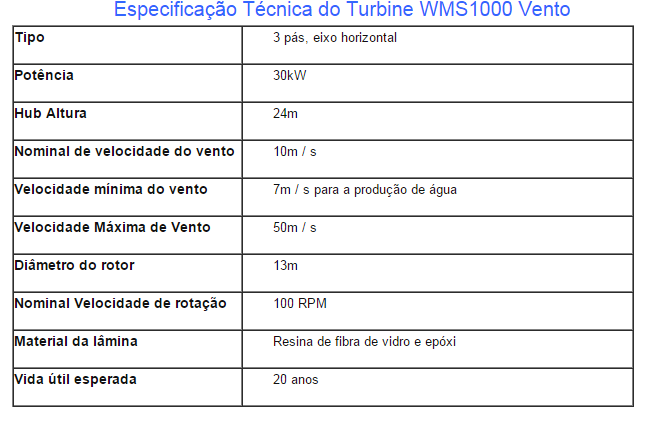
\includegraphics[scale=0.8]{editaveis/figuras/especificacao}
\caption[Especificação Técnica do Turbine WMS1000]{Especificação Técnica do Turbine WMS1000 Vento \footnotemark}
\FloatBarrier
\label{Especificacoes}
\end{figure}
\footnotetext{Fonte: \cite{renewable}}
 
A outra tecnologia, Warawater, por sua vez é uma tecnologia muito barata se comparada com a mencionada anterior. 
Essa custa cerca de US\$ 500 e pode ser construída em menos de uma semana com uma equipe de quatro pessoas e materiais 
existente localmente \cite{warkawater}.

Os materiais necessários para a sua construção de sua estrutura são: recipiente de coleta, bambu e um revestimento
interno de plástico reciclado (rede). Sua torre possui em média 10 metros de altura, com 60 Kg e pode suprir até 100 litros
de água por dia \cite{warkawater2}.

\begin{figure}[!htbp]
\centering
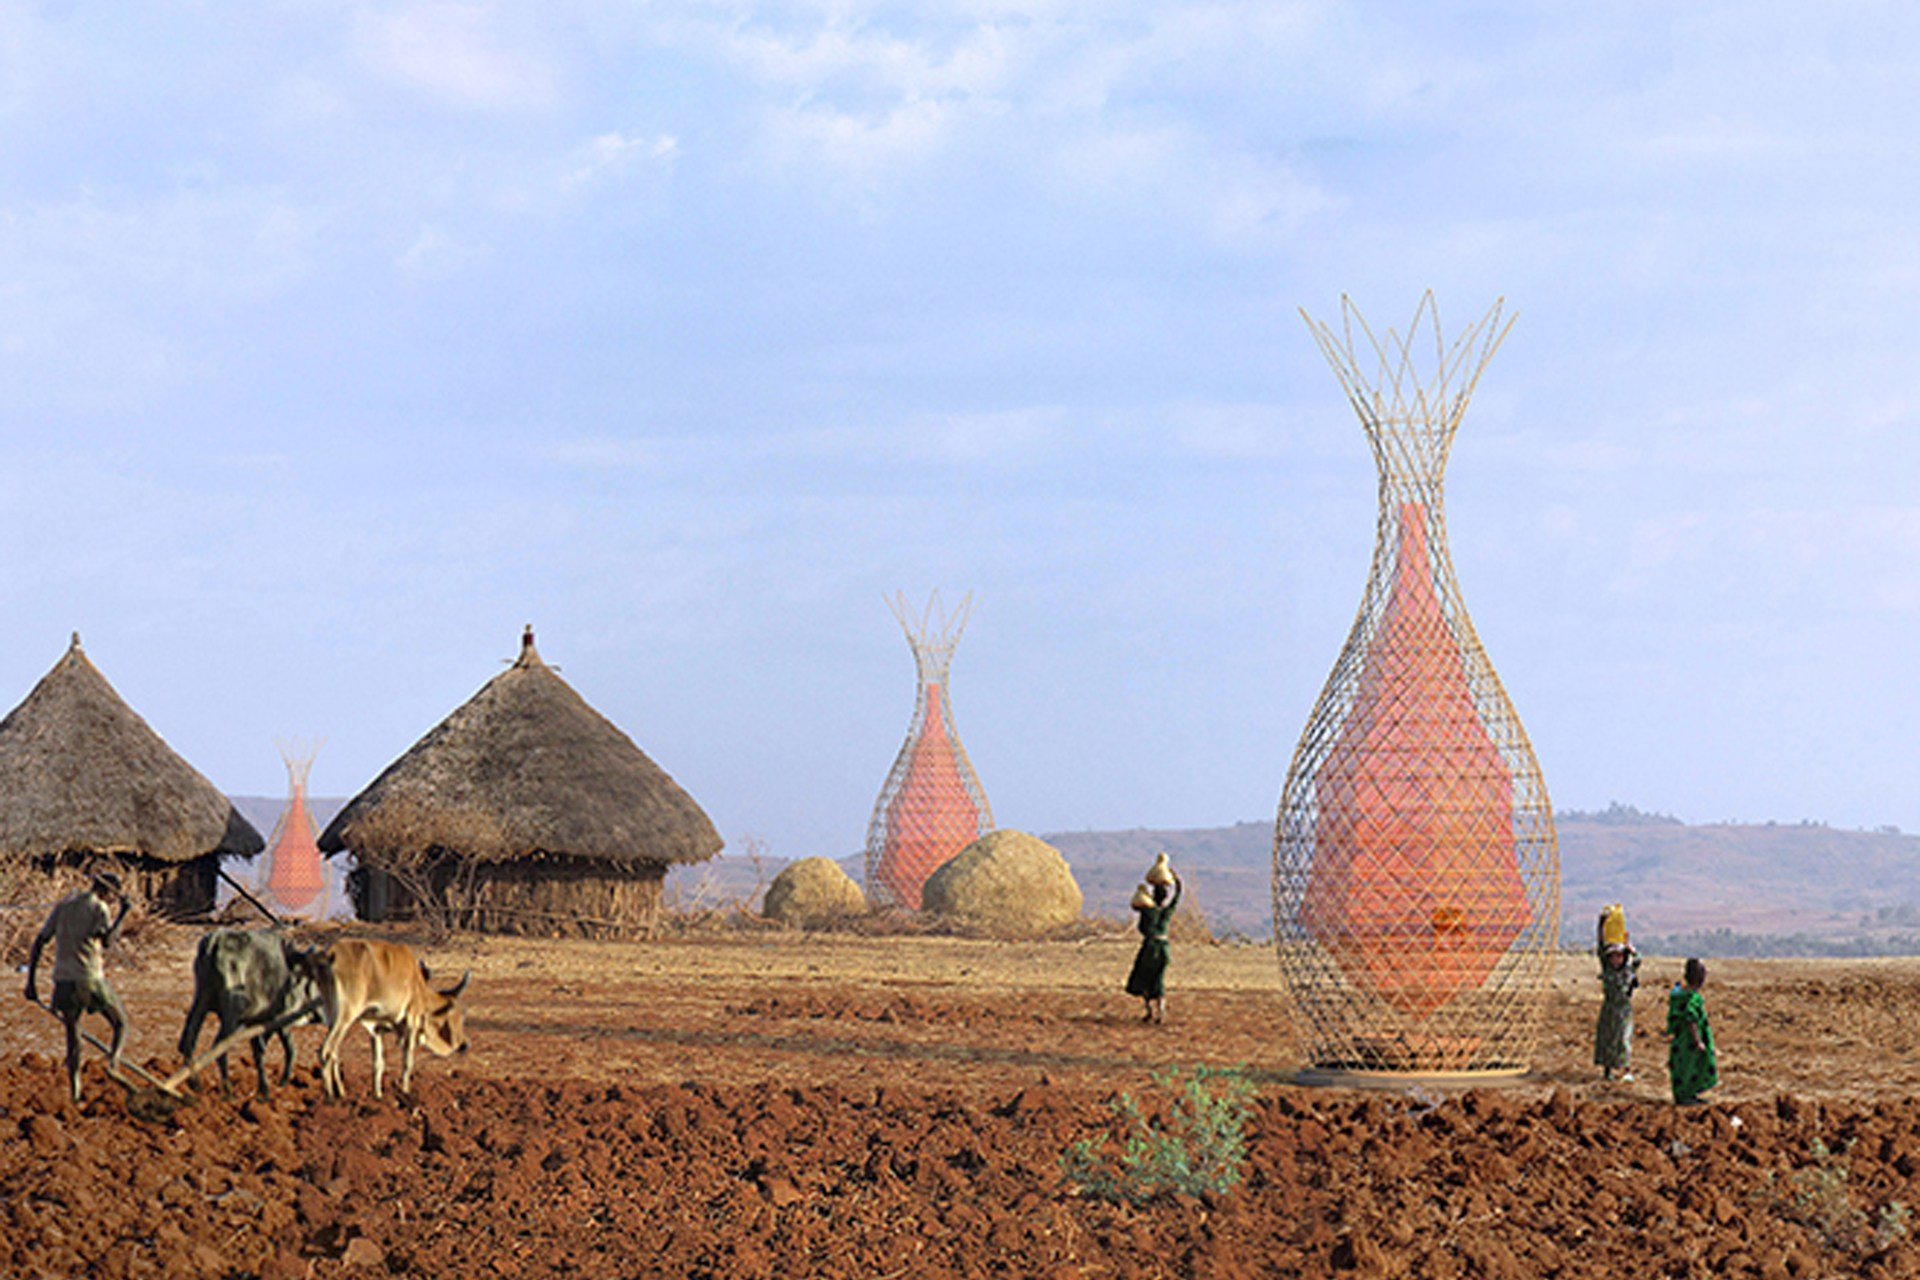
\includegraphics[scale=0.3]{editaveis/figuras/warkawater}
\caption[Utilização da tecnologia warkawater por uma população carente]
{Utilização da tecnologia warkawater por uma população carente  \footnotemark}
\FloatBarrier
\label{Especificacoes}
\end{figure}
\footnotetext{Fonte: \cite{warkawater}}

% \bibliographystyle{abnt-alf}
% \bibliography{bibliografia}

% \end{document}